%% abtex2-modelo-trabalho-academico.tex, v-1.7.1 laurocesar
%% Copyright 2012-2013 by abnTeX2 group at http://abntex2.googlecode.com/
%%
%% This work may be distributed and/or modified under the
%% conditions of the LaTeX Project Public License, either version 1.3
%% of this license or (at your option) any later version.
%% The latest version of this license is in
%% http://www.latex-project.org/lppl.txt
%% and version 1.3 or later is part of all distributions of LaTeX
%% version 2005/12/01 or later.
%%
%% This work has the LPPL maintenance status `maintained'.
%%
%% The Current Maintainer of this work is the abnTeX2 team, led
%% by Lauro César Araujo. Further information are available on
%% http://abntex2.googlecode.com/
%%
%% This work consists of the files abntex2-modelo-trabalho-academico.tex,
%% abntex2-modelo-include-comandos and abntex2-modelo-references.bib
%%

% ------------------------------------------------------------------------
% ------------------------------------------------------------------------
% abnTeX2: Modelo de Trabalho Academico (tese de doutorado, dissertacao de
% mestrado e trabalhos monograficos em geral) em conformidade com
% ABNT NBR 14724:2011: Informacao e documentacao - Trabalhos academicos -
% Apresentacao
% ------------------------------------------------------------------------
% ------------------------------------------------------------------------

\documentclass[
	% -- opções da classe memoir --
	12pt,			% tamanho da fonte
	openright,		% capítulos começam em pág ímpar (insere página vazia caso preciso)
	oneside,			% para impressão em verso e anverso. Oposto a oneside
	a4paper,			% tamanho do papel.
	% -- opções da classe abntex2 --
	chapter=TITLE,		% títulos de capítulos convertidos em letras maiúsculas
	%section=TITLE,		% títulos de seções convertidos em letras maiúsculas
	%subsection=TITLE,	% títulos de subseções convertidos em letras maiúsculas
	%subsubsection=TITLE,% títulos de subsubseções convertidos em letras maiúsculas
	% -- opções do pacote babel --
	english,			% idioma adicional para hifenização
%	spanish,			% idioma adicional para hifenização
	brazil,			% o último idioma é o principal do documento
	]{abntex2}


% ---
% PACOTES
% ---

% ---
% 2Pacotes fundamentais
% ---
\usepackage[brazil]{babel}
\selectlanguage{brazil}
\usepackage{cmap}			% Mapear caracteres especiais no PDF
\usepackage{lmodern}			% Usa a fonte Latin Modern			
\usepackage[T1]{fontenc}		% Selecao de codigos de fonte.
\usepackage[utf8]{inputenc}	% Codificacao do documento (conversão automática dos acentos)
\usepackage{lastpage}			% Usado pela Ficha catalográfica
\usepackage{indentfirst}		% Indenta o primeiro parágrafo de cada seção.
\usepackage{color}			% Controle das cores
\usepackage{graphicx}			% Inclusão de gráficos
\usepackage{float}
\usepackage{longtable}

% ---


% ---
% Pacotes de citações
% ---
\usepackage[brazilian,hyperpageref]{backref}	 % Paginas com as citações na bibl
\usepackage[alf]{abntex2cite}				% Citações padrão ABNT

% ---
% CONFIGURAÇÕES DE PACOTES
% ---

% ---
% Configurações do pacote backref
% Usado sem a opção hyperpageref de backref
\renewcommand{\backrefpagesname}{Citado na(s) página(s):~}
% Texto padrão antes do número das páginas
\renewcommand{\backref}{}
% Define os textos da citação
\renewcommand*{\backrefalt}[4]{
	\ifcase #1 %
		Nenhuma citação no texto.%
	\or
		Citado na página #2.%
	\else
		Citado #1 vezes nas páginas #2.%
	\fi}%
% ---


% ---
% Informações de dados para CAPA e FOLHA DE ROSTO
% ---
\titulo{DESENVOLVIMENTO DE TECNOLOGIA FOCADO EM IHC}

\autor{
Guilherme Anderzen Polido
}
\local{TOLEDO, PR}
\data{2019}

\orientador{Eduardo Pezutti Beletato dos Santos}

\instituicao{
UNIVERSIDADE TECNOLÓGICA FEDERAL DO PARANÁ \par
CAMPUS TOLEDO \par
COORDENAÇÃO DO CURSO DE TECNOLOGIA EM SISTEMAS PARA INTERNET
% \par
% Design Digital
% \par
% Programa de Graduação
}
\tipotrabalho{Trabalho de conclusão de curso}
% O preambulo deve conter o tipo do trabalho, o objetivo,
% o nome da instituição e a área de concentração
\preambulo{Trabalho de Conclusão de Curso de Graduação, apresentado ao Curso Superior de Tecnologia em Sistemas para Internet, da Universidade Tecnológica Federal do Paraná – UTFPR, como requisito parcial para obtenção do título de Tecnólogo. Orientador: Prof. \imprimirorientador}
% ---


% ---
% Configurações de aparência do PDF final

% alterando o aspecto da cor azul
%\definecolor{blue}{RGB}{41,5,195}
\definecolor{blue}{RGB}{0,0,0}

% informações do PDF
\makeatletter
\hypersetup{
	%pagebackref=true,
	pdftitle={\@title},
	pdfauthor={\@author},
	pdfsubject={\imprimirpreambulo},
	pdfcreator={LaTeX with abnTeX2},
	pdfkeywords={abnt}{latex}{abntex}{abntex2}{trabalho acadêmico},
	colorlinks=true, 	% false: boxed links; true: colored links
	linkcolor=blue, 	% color of internal links
	citecolor=blue, 	% color of links to bibliography
	filecolor=magenta, 	% color of file links
	urlcolor=blue,
	bookmarksdepth=4
}
\makeatother
% ---

% ---
% Espaçamentos entre linhas e parágrafos
% ---

% O tamanho do parágrafo é dado por:
\setlength{\parindent}{1.3cm}

% Controle do espaçamento entre um parágrafo e outro:
\setlength{\parskip}{0.2cm} % tente também \onelineskip

% ---
% compila o indice
% ---
\makeindex
% ---

% ----
% Início do documento
% ----
\begin{document}

% Retira espaço extra obsoleto entre as frases.
\frenchspacing

% ----------------------------------------------------------
% ELEMENTOS PRÉ-TEXTUAIS
% ----------------------------------------------------------
% \pretextual

% ---
% Capa
% ---
\imprimircapa
% ---

% ---
% Folha de rosto
% (o * indica que haverá a ficha bibliográfica)
% ---
\imprimirfolhaderosto*
% ---

% ---
% Inserir a ficha bibliografica
% ---

% Isto é um exemplo de Ficha Catalográfica, ou ``Dados internacionais de
% catalogação-na-publicação''. Você pode utilizar este modelo como referência.
% Porém, provavelmente a biblioteca da sua universidade lhe fornecerá um PDF
% com a ficha catalográfica definitiva após a defesa do trabalho. Quando estiver
% com o documento, salve-o como PDF no diretório do seu projeto e substitua todo
% o conteúdo de implementação deste arquivo pelo comando abaixo:

% \begin{fichacatalografica}
% \includepdf{fig_ficha_catalografica.pdf}
% \end{fichacatalografica}

%\begin{fichacatalografica}
%	\vspace*{\fill}					% Posição vertical
%	\hrule						% Linha horizontal
%	\begin{center}				% Minipage Centralizado
%	\begin{minipage}[c]{12.5cm}	% Largura
%	
%	\imprimirautor
%	
%	\hspace{0.5cm} \imprimirtitulo / \imprimirautor. --
%	\imprimirlocal, \imprimirdata-
%	
%	\hspace{0.5cm} \pageref{LastPage} p. : il. (algumas color.) ; 30 cm.\\
%	
%	\hspace{0.5cm} \imprimirorientadorRotulo~\imprimirorientador\\
%	
%	\hspace{0.5cm}
%	\parbox[t]{\textwidth}{\imprimirtipotrabalho~--~\imprimirinstituicao,
%	\imprimirdata.}\\
%	
%	\hspace{0.5cm}
%		1. Palavra-chave1.
%		2. Palavra-chave2.
%		I. Orientador.
%		II. Universidade xxx.
%		III. Faculdade de xxx.
%		IV. Título\\ 			
%	
%	\hspace{8.75cm} CDU 02:141:005.7\\
%	
%	\end{minipage}
%	\end{center}
%	\hrule
%\end{fichacatalografica}
% ---

% ---
% Inserir errata
% ---
%%\begin{errata}
%%Elemento opcional da \citeonline[4.2.1.2]{NBR14724:2011}. Exemplo:
%%
%%\vspace{\onelineskip}
%%
%%FERRIGNO, C. R. A. \textbf{Tratamento de neoplasias ósseas apendiculares com
%%reimplantação de enxerto ósseo autólogo autoclavado associado ao plasma
%%rico em plaquetas}: estudo crítico na cirurgia de preservação de membro em
%%cães. 2011. 128 f. Tese (Livre-Docência) - Faculdade de Medicina Veterinária e
%%Zootecnia, Universidade de São Paulo, São Paulo, 2011.
%%
%%\begin{table}[htb]
%%\center
%%\footnotesize
%%\begin{tabular}{|p{1.4cm}|p{1cm}|p{3cm}|p{3cm}|}
%% \hline
%% \textbf{Folha} & \textbf{Linha} & \textbf{Onde se lê} & \textbf{Leia-se} \\
%% \hline
%% 1 & 10 & auto-conclavo & autoconclavo\\
%% \hline
%%\end{tabular}
%%\end{table}
%%
%%\end{errata}
% ---

% ---
% Inserir folha de aprovação
% ---

% Isto é um exemplo de Folha de aprovação, elemento obrigatório da NBR
% 14724/2011 (seção 4.2.1.3). Você pode utilizar este modelo até a aprovação
% do trabalho. Após isso, substitua todo o conteúdo deste arquivo por uma
% imagem da página assinada pela banca com o comando abaixo:
%
%
%\begin{folhadeaprovacao}
%
% \begin{center}
% {\ABNTEXchapterfont\large\imprimirautor}
%
% \vspace*{\fill}\vspace*{\fill}
% {\ABNTEXchapterfont\bfseries\Large\imprimirtitulo}
% \vspace*{\fill}
%
% \hspace{.45\textwidth}
%
%
%%{\large COMISSÃO JULGADORA}
%%
%%{\large MONOGRAFIA PARA A CONCLUSÃO DO CURSO\\DE DESIGN DIGITAL}
%
%
% \assinatura{\textbf{\imprimirorientador} \\ Presidente e Orientador}
%% \assinatura{\textbf{Professor} \\ 2º Examinador}
%% \assinatura{\textbf{Professor} \\ 3º Examinador}
%
%
%
%
% \begin{center}
% \vspace*{0.5cm}
% {\large Araraquara, \today}
% \vspace*{1cm}
% \end{center}
%
%\end{folhadeaprovacao}
% ---

% ---
% Dedicatória
% ---
%%\begin{dedicatoria}
%% \vspace*{\fill}
%% \centering
%% \noindent
%% \textit{ Este trabalho é dedicado às crianças adultas que,\\
%% quando pequenas, sonharam em se tornar cientistas.} \vspace*{\fill}
%%\end{dedicatoria}
% ---

% ---
% Agradecimentos
% ---
%\begin{agradecimentos}
%
%
%
%
%\end{agradecimentos}
% ---

% ---
% Epígrafe
% ---
% \begin{epigrafe}
% \vspace*{\fill}
% 	\begin{flushright}
% 		\textit{``Não vos amoldeis às estruturas deste mundo, \\
% 		mas transformai-vos pela renovação da mente, \\
% 		a fim de distinguir qual é a vontade de Deus: \\
% 		o que é bom, o que Lhe é agradável, o que é perfeito.\\
% 		(Bíblia Sagrada, Romanos 12, 2)}
% 	\end{flushright}
% \end{epigrafe}
% ---

% ---
% RESUMOS
% ---

% resumo em português
\begin{resumo}
	A área de tecnologia assistiva surgiu para possibilitar que pessoas com algum tipo de deficiência física ou motora tenham uma vida autônoma, oferecendo alguns recursos, produtos ou até mesmo métodos para auxiliá-los. Esse trabalho tem o objetivo de criar controles para computador voltados para tecnologia assistiva, e IHC (Interação Humano Computador). Para atingir esse objetivo serão realizados testes de usabilidade com pessoas portadoras de algum tipo de deficiência física ou motora a qual dificulte ou até mesmo impossibilite o uso do computador. Os controles serão construídos com materiais de fácil manuseio presentes no mercado atual.

\vspace{\onelineskip}
\noindent
\textbf{Palavras-chaves}: Tecnologia Assistiva, Usabilidade, Deficiência Física, IHC.
\end{resumo}

% resumo em inglês
\begin{resumo}[Abstract]
\begin{otherlanguage*}{english}
Write Abstract

\vspace{\onelineskip}
\noindent
\textbf{Key-words}: .
\end{otherlanguage*}
\end{resumo}
% ---

% ---
% inserir lista de ilustrações
% ---
\pdfbookmark[0]{\listfigurename}{lof}
\listoffigures*
\cleardoublepage
% ---

% ---
% inserir lista de tabelas
% ---
\pdfbookmark[0]{\listtablename}{lot}
\listoftables*
\cleardoublepage
% ---

% ---
% inserir lista de abreviaturas e siglas
% ---
%%%\begin{siglas}
%%% \item[Fig.] Area of the $i^{th}$ component
%%% \item[456] Isto é um número
%%% \item[123] Isto é outro número
%%% \item[lauro cesar] este é o meu nome
%%%\end{siglas}
% ---

% ---
% inserir lista de símbolos
% ---
%%%\begin{simbolos}
%%% \item[$ \Gamma $] Letra grega Gama
%%% \item[$ \Lambda $] Lambda
%%% \item[$ \zeta $] Letra grega minúscula zeta
%%% \item[$ \in $] Pertence
%%%\end{simbolos}
% ---

% ---
% inserir o sumario
% ---
\pdfbookmark[0]{\contentsname}{toc}
\tableofcontents*
\cleardoublepage
% ---



% ----------------------------------------------------------
% ELEMENTOS TEXTUAIS
% ----------------------------------------------------------
\textual

% ----------------------------------------------------------
% Introdução
% ----------------------------------------------------------
\chapter[Introdução]{Introdução}

Segundo a cartilha do censo 2010 pessoas com deficiência no Brasil (2012) 23,9\% da população possui algum tipo de deficiência que pode ser: visual, auditiva, motora e mental ou intelectual. A deficiência visual prevalece com um total de 18,6\%, em segundo lugar foi destacado a deficiência motora com 7\%, seguida da auditiva com 5,10\% e mental ou intelectual em 1,40\%.

Segundo \cite{lazarojcs} a deficiência motora é uma disfunção de caráter congênito ou adquirido. Uma das causas da deficiência motora mais recorrente é a paralisia cerebral. Muitas pessoas com paralisia cerebral são capazes de usar computadores, mas geralmente encontram dificuldade para usar um mouse. Os movimentos dos braços muitas vezes são demasiadamente irregulares e imprevisíveis para usar um mouse de maneira eficaz. A \cite{utah}, uma organização sem fins lucrativos que fornece soluções em acessibilidade web, diz que normalmente estas pessoas podem fazer uso de teclado para simular um mouse, ou até mesmo um teclado adaptado para elas, embora mais lentamente do que pessoas que não possuem paralisia cerebral.

Algumas deficiências e/ou doenças como paralisia cerebral, esclerose múltipla ou lateral, artrite e mal de Parkinson podem impossibilitar a realização de atividades que necessitam das mãos, como utilizar um computador, causando movimentos imprevisíveis, tremores, rigidez muscular entre outros.

O surgimento da área de tecnologia assistiva, se deu devido a necessidade de inclusão dessas pessoas com algum tipo de impossibilidade motora a sociedade em geral. Ou seja, a tecnologia assistiva apresenta uma série de produtos, recursos, metodologias e práticas a fim de promover a autonomia desses indivíduos dentro da sociedade em que está inserido. Com a tecnologia assistiva a utilização de computadores por essas pessoas torna-se recorrente. Porém o custo de um equipamento com essa finalidade normalmente é alto, e nem todos possuem condições para adquiri-los.

No mercado é possível encontrar alguns controles para deficientes físicos, como por exemplo o Tix (Figura \ref{img:img-14-2}), desenvolvido no Brasil, possui botões que quando combinados formam comandos específicos, como alguma letra do alfabeto, ou ativar a movimentação do ponteiro do mouse, entre outros.

\begin{figure}[H]
\centering
		\includegraphics[width=0.8\textwidth]{./img/img-14.png}
		\caption{Teclado Tix}
		\label{img:img-14-2}
\end{figure}

Na computação existe a área de IHC (Interface Homem Computador), a qual tem o objetivo de estudar as formas que humanos interagirem com um computador. Ou seja, estuda a interface pela qual usuários interagem com o computador, seja ela páginas web, teclados adaptativos para deficientes físicos, entre outros. Além disso a área de IHC oferece várias formas de realizar testes unitários a fim de avaliar a experiência do usuário com aquela interface desenvolvida.

O objetivo deste trabalho é realizar um estudo baseado em IHC a fim de destacar o que é necessário para desenvolver controles voltados para tecnologia assistiva com materiais acessíveis. Para alcançar esse objetivo serão definidos os principais comandos que devem existir nesses controles e quais materiais serão necessários. Após isso os controles serão construídos seguindo o que foi estudado até então e por fim avaliar se o estudo obteve bons resultados ou não.

\section{Objetivos}
\label{obj}

\subsection{Objetivo Geral}
Criar controles voltados para tecnologia assistiva utilizando IHC, materiais acessíveis, facilidade de construção e integração com o computador.

\subsection{Objetivos Específicos}
\begin{itemize}
	\item Definir o conjunto de comandos que serão implementados nos controles.
	\item Definir os materiais necessários de forma ue seja fácial a sua montagem.
	\item Realizar e avaliar testes com pessoas portadoras de alguma deficiência física.
	\item Montar os controles e realizar os testes finais para validá-los.
\end{itemize}


% ---
% Capitulo de revisão de literatura
% ---
\chapter{Referencial Teórico}
\label{refteo}

Nesta seção serão apresentados conceitos importantes para o esclarecimento do tema abordado nesse texto, a fim de estabelecer um entendimento comum entre os itens que serão apresentados.

\section{Interação Humano Computador}

Na área de IHC podemos encontrar alguns termos como usabilidade, ergonomia, aprendizagem, acessibilidade e interatividade, os quais são definidos como:

\subsection{Usabilidade}

A ABNT NBR ISO 9241-11 \(ref 5 de Garbin Sander Maeda.pdf\) define usabilidade como modo que um produto pode ser utilizado por usuários, a fim de alcançar os objetivos específicos com sucesso, eficiência e satisfação em um contexto de uso. Assim um sistema interativo deve considerar que a utilização deve ser eficaz para seu usuário alvo, levando em consideração que ele pode ou não ter familiaridade com o dispositivo, ou similar a ele. A interação com usuários deve ser fácil e intuitiva levando em conta a ergonomia e interfaces simples para o usuário.

A norma NBR ISSO/IEC 9126-1 \(ref 6 de Garbin Sander Maeda.pdf\) declara algumas características que um sistema com uma boa usabilidade de conter, são elas:

\begin{itemize}
	\item Inteligibilidade:

É a facilidade em que o usuário do sistema compreende as funcionalidades e consegue definir se pode ser usado para realizar as tarefas que ele pretende fazer.

\item Apreensibilidade:

É considerado como a facilidade com que o usuário aprende a utilizar o sistema.

\item Operacionalidade:

É como o sistema facilita que o usuário o opere, incluindo como ele trata as falhas e erros que podem surgir nas operações.

\item Atratividade:

Modo utilizado para atrair novos usuários para o sistema, podendo ser desde a adaptação das operações para usuário, até mesmo melhorias visuais na interface para melhor atender o usuário.

\end{itemize}

\subsection{Ergonomia}

Segundo Wisner \(Ref 9 de Garbin Sander Maeda.pdf\) ergonomia é definida como um conjunto de conhecimentos científicos relacionados ao homem e a instrumentos, máquinas e dispositivos que serão utilizados, levando em conta o máximo de conforto, segurança e eficiência.

Ao se construir um dispositivo deve ser levado em consideração o comportamento físico e mental de como o homem interage com o mesmo. Então esse dispositivo além de ser flexível o suficiente, a fim de se adequar a diferentes usuários, também deve ser amigável e confortável, tanto para novos usuários quanto para os quais já estão familiarizados com o seu funcionamento e modo de operação.

\subsection{Aprendizagem}

É o processo pelo qual se adquire conhecimentos, habilidades e valores como benefício de um estudo, experiência ou observação. Esse conceito está ligado com a usabilidade, pois se ela estiver inadequada para o usuário sua curva de aprendizagem e a quantidade de erros serão maiores do que um dispositivo com uma boa usabilidade.

Uma maior curva de aprendizagem e de erros, levam a um maior número de modificações ou até mesmo duplicidade de funções a fim de melhorar a usabilidade, o que requer maior esforço do usuário para reaprender muitas coisas, levando assim a frustração do mesmo, e por fim uma imagem negativa do produto.

\subsection{Acessibilidade}

A Lei nº 10.098, de dezembro de 2000 define acessibilidade como:

\begin{quote}\small\setlength{\leftskip}{4cm}
Possibilidade e condição de alcance para utilização, com segurança e autonomia, dos espaços, mobiliários e equipamentos urbanos, das edificações, dos transportes e dos sistemas e meios de comunicação, por pessoa portadora de deficiência ou com mobilidade reduzida.
\end{quote}

É essencial garantir a acessibilidade para todos de forma que possibilite a melhoria da qualidade de vida das pessoas. Atualmente a acessibilidade está sendo aplicada em diversos contextos, desde de construção civil, equipamento domésticos, computadores, escolas, transporte, entre outros.

\subsection{Interatividade}

Para que aconteça a comunicação entre humano e computador, é necessário que exista um meio de troca de informações. Então para que ocorra a iteração é necessário de dispositivos de entrada, os quais possibilitam a entrada de dados do usuário para a máquina, e de saída, ou seja a resposta da máquina para o usuário.

Além dos dispositivos de entrada e saída também é importante que a ergonomia do equipamento seja adequada, e possibilita adaptar-se a diferentes tipos de usuários, garantindo uma interação agradável e positiva.

\section{Tecnologia assistiva}

Em meio à era digital, em que o desenvolvimento de novas tecnologias se torna algo acelerado, é importantíssimo que a sociedade esteja pronta para adaptação de todos os indivíduos a cultura digital. Segundo \cite{castrota} percebermos que a evolução tecnológica torna a vida das pessoas mais fácil, indiferente do ambiente em que ela está inserida. Para eles, sem notarmos, usufruímos diariamente ferramentas desenvolvidas para facilitar as atividades rotineiras, como computadores, celulares, controles remotos, veículos, e uma interminável lista de meios tecnológicos, que são parte de nosso dia a dia.

Em 14 de dezembro de 2007, o CAT (COMITÊ DE AJUDAS TÉCNICAS) aprovou, o seguinte conceito para TA (TECNOLOGIA ASSISTIVA):

\begin{quote}\small\setlength{\leftskip}{4cm}
Tecnologia Assistiva é uma área do conhecimento, de característica interdisciplinar, que engloba produtos, recursos, metodologias, estratégias, práticas e serviços que objetivam promover a funcionalidade, relacionada à atividade e participação, de pessoas com deficiência, incapacidades ou mobilidade reduzida, visando sua autonomia, independência, qualidade de vida e inclusão social (Comitê de Ajudas Técnicas – ATA VI). \citeonline{assistiva}
\end{quote}

A área de TA é classificada de acordo com os objetivos a que se destinam. A classificação a ser apresentada na tabela \ref{tab:tab-1}, a qual foi escrita por José Tonolli e Rita Bersch em 1998.

\begin{table}[H]
\caption{Classificações da área de Tecnologia Assistiva}
\label{tab:tab-1}
{
\centering
\footnotesize
\begin{tabular}{|p{7cm}|p{7cm}|}
\hline
\textbf{BD Relacionais} & \textbf{BD Orientados a Objetos} \\
\hline
Auxílios para a vida diária e vida prática & Materiais e produtos que favorecem desempenho autônomo e independente em tarefas rotineiras.\\
\hline
Comunicação Aumentativa e Alternativa (CAA) & Destinada a atender pessoas sem fala ou escrita funcional ou em defasagem entre sua necessidade comunicativa e sua habilidade em falar e/ou escrever.\\
\hline
Recursos de acessibilidade ao computador & Conjunto de hardware e software especialmente idealizado para tornar o computador acessível a pessoas com privações sensoriais (visuais e auditivas),intelectuais e motoras. Inclui dispositivos de entrada (mouses, teclados e acionadores diferenciados) e dispositivos de saída (sons, imagens, informações táteis).\\
\hline
Sistemas de controle de ambiente & Controles que são programados para realizar funções (apagar ou acender luzes, desligar fogo ou torneira, trancar ou abrir portas, etc.) e promover maior independência.\\
\hline
Projetos arquitetônicos para acessibilidade & Projetos de edificação e urbanismo que garantem acesso físico.\\
\hline
Órteses e próteses & Próteses são peças artificiais que substituem partes ausentes do corpo. Órteses são colocadas junto a um segmento corpo, garantindo-lhe um melhor posicionamento, estabilização e/ou função.\\
\hline
Adequação Postural & Recursos que ajudem os sujeitos a ter uma postura estável e confortável, favorecendo um bom desempenho funcional.\\
\hline
Auxílios de mobilidade & Recursos utilizados para auxiliar na mobilidade dos sujeitos.\\
\hline
Auxílios para qualificação da habilidade visual e recursos que ampliam a informação às pessoas com deficiência visual & Equipamentos que visam à independência das pessoas com deficiência visual na realização de tarefas diárias.\\
\hline
Auxílios para pessoas com deficiência auditiva & Equipamentos que visam à independência das pessoas com deficiência auditiva na realização das suas tarefas.\\
\hline
Mobilidade em veículos & São adaptações realizadas em veículos para auxiliar no deslocamento da pessoa com deficiência.\\
\hline
Esporte e Lazer & Recursos que favorecem a prática de esporte e participação em atividades de lazer.\\
\hline
\end{tabular}
}
\end{table}

Os recursos de acessibilidade ao computador tendem a tornar a experiência do usuário, portador de alguma deficiência física, a qual implica na utilização do computador, mais fácil e inclusiva. Tendo em mente que existem várias deficiências, e que em cada uma delas é necessário um tipo de adaptação específica, são desenvolvidos diferentes recursos que podemos chamar de equipamentos, se essa divisão não ocorresse, tornaria o projeto de desenvolvimento do mesmo muito custoso e complexo.

Alguns equipamentos classificados como recursos de acessibilidade ao computador por Tonolli e Bersh são:

\textbf{Ponteiras de Cabeça}

Ferramentas que são fixadas à cabeça, e auxiliam, o uso do teclado, como podemos ver na figura \ref{img:img-12}:

\begin{figure}[H]
	\centering
		\includegraphics[width=0.7\textwidth]{./img/img-12.jpg}
		\caption{Ferramenta de ponteira}
		\label{img:img-12}
\end{figure}

\textbf{Teclados Especiais}

Dispositivos de hardware ou de software que oferecem uma alternativa para a utilização das teclas, ou seja, simulam o funcionamento do teclado. Como teclados com teclas maiores (Figura \ref{img:img-5}), protetores para as teclas (Figura \ref{img:img-7}) e softwares que simulam o teclado na tela do computador (Figura \ref{img:img-6}).

\begin{figure}[H]
	\centering
		\includegraphics[width=0.5\textwidth]{./img/img-5.png}
		\caption{Teclados com teclas maiores}
		\label{img:img-5}
\end{figure}

\begin{figure}[H]
	\centering
		\includegraphics[width=0.5\textwidth]{./img/img-7.jpg}
		\caption{Protetor para as teclas}
		\label{img:img-7}
\end{figure}

\begin{figure}[H]
	\centering
		\includegraphics[width=0.5\textwidth]{./img/img-6.png}
		\caption{Teclado Virtual}
		\label{img:img-6}
\end{figure}

\textbf{Mouses Adaptados}

Dispositivos de hardware, que possibilita o movimento preciso do cursor na tela, utilizado por pessoas com dificuldades motoras, mesmo que com habilidades motoras reduzidas, simulando as mesmas funções encontradas num mouse convencional, como o Trackball (Figura \ref{img:img-8}), Roller Mouse (Figura \ref{img:img-9}).

No Trackball a pessoa utiliza as mãos para girar a esfera e movimentar o mouse, e pode utilizar os outros botões para ações como click direto e esquerdo do mouse.

\begin{figure}[H]
	\centering
		\includegraphics[width=0.5\textwidth]{./img/img-8.jpg}
		\caption{Trackball}
		\label{img:img-8}
\end{figure}

No Roller Mouse, o usuário utiliza os pés para girar os dois rolos responsáveis pela movimentação do mouse, e os botões para outras funções que pode ser encontrado no mouse convencional.

\begin{figure}[H]
	\centering
		\includegraphics[width=0.5\textwidth]{./img/img-9.jpg}
		\caption{Roller Mouse}
		\label{img:img-9}
\end{figure}

Em 2015 a empresa brasileira TIX, lançou um produto chamado de Teclado Inteligente Multifuncional TiX (Figura \ref{img:img-14}), dando origem a muitos outros acessórios e aplicativos de Tecnologia Assistiva. Esse equipamento, possui botões que ao serem combinados formam comandos específicos, podendo ser uma letra do alfabeto, ou até mesmo ativar a movimentação do ponteiro do mouse.

\begin{figure}[H]
	\centering
		\includegraphics[width=0.7\textwidth]{./img/img-14.png}
		\caption{TIXX}
		\label{img:img-14}
\end{figure}

\section{Plataforma ARDUINO®}

O ARDUINO® é uma plataforma de hardware livre criado no ano de 2005 pelos pesquisadores Massimo Banzi, David Cuartielles, Tom Igoe, Gianluca Martino e David Mellis com o objetivo de desenvolver uma plataforma de desenvolvimento barato, funcional e de fácil programação, tornando possível que qualquer pessoa mesmo as que possuem pouco conhecimento de eletrônica, possa utilizar essa plataforma. Na Figura \ref{img:img-16} pode-se ver uma placa de ARDUINO® modelo UNO.

\begin{figure}[H]
	\centering
		\includegraphics[width=0.7\textwidth]{./img/img-16.png}
		\caption{Placa ARDUINO® Uno}
		\label{img:img-16}
\end{figure}

As placas ARDUINO® possuem microcontroladores Atmel, com circuitos de entrada e saída prontos, e pode ser facilmente programada via computador utilizando um cabo USB. A programação do microcontrolador é baseada na linguagem C/C++, e após programado pode funcionar de forma independente, controlando um robô, acendendo e apagando luzes, ligando motores, recebendo comandos e os enviando para o computador, entre outros.

O ARDUINO® pode fazer inúmeras funções, ou ser aplicado em diversos contextos, como automatização de uma casa, de um carro, criar brinquedos, robôs, controlador para máquinas de corte, joystick, e várias outras coisas. Além da placa ARDUINO® existem vários outros módulos que podem ser associados a ela, como módulos relés, sensores de luz, som, chuva, temperatura entre outros.

Além desses módulos existem placas chamadas de Shields, as quais podem ser acopladas ao ARDUINO® e aumentar o número de funcionalidades do mesmo. Um exemplo é a placa “ARDUINO® Ethernet Shield”, o qual possibilita conexão com a internet via cabo de rede. Na Figura \ref{img:img-15} pode-se ver uma placa ARDUINO® Mega, com uma Ethernet Shield acoplada.

\begin{figure}[H]
	\centering
		\includegraphics[width=0.7\textwidth]{./img/img-15.png}
		\caption{Placa ARDUINO® Mega}
		\label{img:img-15}
\end{figure}

Para facilitar ainda mais também foi criado uma IDE (Ambiente Integral de Desenvolvimento) para programação da placa, a qual conta com todos os recursos necessários para se desenvolver um projeto nessa plataforma, como exemplos prontos, bibliotecas, realização de testes no código antes de ser carregado e transferência do programa para a placa de forma muito fácil.

Hoje existem inúmeros modelos de placas ARDUINO® no mercado, algumas com o mesmo microcontrolador porém com tamanho reduzido. Normalmente o que altera de um para outro é a quantidade de portas disponíveis para utilizar, microcontrolador utilizado, quantidade de memória disponível, velocidade de processamento, tipo de conexão, tensão suportada e corrente entregue pelas portas. A tabela \ref{tab:tab-2} mostra as especificações de alguns modelos de ARDUINO® mais conhecidos.

\begin{table}[H]
\caption{Especificações de placas ARDUINO® mais conhecidas}
\label{tab:tab-2}
{
\centering
\footnotesize
\begin{tabular}{|p{5cm}|p{2cm}|p{2cm}|p{3cm}|p{2cm}|}
\hline
\textbf{Modelos} & UNO & MEGA & LEONARDO & NANO \\
\hline
Microcontrolador & Atmega 328 & Atmega 2560 & Atmega 32U4 & Atmega 328 \\
\hline
Portas Digitais & 14 & 54 & 20 & 14 \\
\hline
Portas PWM & 6 & 15 & 7 & 6 \\
\hline
Portas Analógicas & 6 & 16 & 12 & 8 \\
\hline
Memoria & 32K & 256K & 32K & 32K \\
\hline
Clock & 16Mhz & 16Mhz & 16Mhz & 16Mhz \\
\hline
Conexão & USB & USB & Micro USB & USB Mini-B \\
\hline
Alimentação externa & Sim & Sim & Sim & Não \\
\hline
Tensão de Operação & 5v & 5v & 5v & 5v \\
\hline
Corrente Máxima por E/S & 40mA & 40mA & 40mA & 40mA \\
\hline
Alimentação & 7-12Vdc & 7-12Vdc & 7-12Vdc & 7-12Vdc\\
\hline
\end{tabular}
}
\end{table}

\section{Biblioteca Unojoy}
O Unojoy é uma biblioteca desenvolvida em C por Alan Chatham e Eero Prittinen, o projeto é de código aberto e está disponível em seus repositórios do github, a sua primeira versão foi liberada em fevereiro de 2014, e a mais recente em março de 2019. A biblioteca possibilita que um ARDUINO® UNO possa ser utilizado como joystick, sem a necessidade de modificar o seu hardware. Essa biblioteca foi desenvolvida comunicação com as plataformas Windows, Linux e OSX.

Depois de preparado e instalada a biblioteca no ARDUINO®, para utilizá-lo em qualquer outro computador basta plugá-lo na porta USB. O driver será instalado sem a necessidade de configurar mais nada, e após isso deve ser utilizado algum software que emula algumas funções do sistema operacional quando pressionar algum botão do joystick.

A tabela \ref{tab:tab-3} mostra alguns softwares capazes de simular essas funções no sistema operacional, relacionando outros fatores como sistemas operacionais suportados, se é um software gratuito e sua última versão disponível.

\begin{table}[H]
\caption{Softwares para simular funções do S.O. usado um \emph{joystick}}
\label{tab:tab-3}
{
\centering
\footnotesize
\begin{tabular}{|p{2cm}|p{3cm}|p{6cm}|p{3cm}|}
\hline
\textbf{Nome} & \textbf{Licença} & \textbf{SOs suportados} & \textbf{Última Versão}\\
\hline
JoyToKey	&30 dias grátis				&Windows 10,8,7, Vista, XP		&6.1.1 - 23/09/2018\\
\hline
Antimicro	&Open Source				&Windows 10,8,7, Vista, XP e Linux.	&2.23 - 06/11/2016\\
\hline
Xpadder	&Pago						&Windows 10,8,7, Vista, XP 		&-\\
\hline
\end{tabular}
}
\end{table}

Ao utilizar o ARDUINO® UNO é necessário carregar o código para ATmega16u2, responsável por gerenciar a comunicação entre o chip controlador Atmega 328p e a porta USB \footnote{Sigla USB, do inglês Universal Serial Bus} do computador, para que o mesmo seja reconhecido como um Joystick ao conectar na porta USB. Diferentemente do ARDUINO® Leonardo, que a comunicação entre o chip controlador Atmega32u4 e a porta USB é feita de forma direta, sem a necessidade de outro circuito integrado como o ATmega8u2 para gerenciar essa comunicação.

Para a construção dos controles pode ser utilizado o ARDUINO® UNO R3, sendo obrigatório que ele possua o micro controlador ATmega8u2, pois a versão chinesa a qual possui o controlador CH340, que também faz o papel de intermediar a comunicação entre o Atmega 328p e a porta USB, não permite programá-lo. Também pode ser utilizado o ARDUINO® Leonardo, pois ele já possui a comunicação integrada no próprio controlador, ou o ARDUINO® MEGA para casos em que serão necessários mais de 13 botões no controle.

\chapter{Metodologia}
\label{met}

Esse trabalho é de natureza qualitativa, na qual se baseou em outro trabalho desenvolvido em 2016 pelo professor orientador em conjunto com outros alunos da UTFPR. Esse trabalho desenvolvido em 2016 abordou durante seu desenvolvimento e testes algumas informações importantes, as quais foram utilizadas para a construção do nosso controle. Durante três anos pessoas com deficiência motora utilizaram esse controle para trabalho, e durante esse tempo, foram levantados algumas possíveis melhorias, as quais foram aplicadas no presente trabalho.

Após a construção dos novos controles foram feitos alguns testes, os quais tiveram resultados positivos. Ao realizar testes com duas pessoas foi possível notar que a regulagem da inclinação do controle foi bem aceita, a utilização do manche, para movimentação do mouse, como descrito pelos participantes do testes, foi fácil e simples. Porém ainda foram encontrados alguns problemas com a fixação dos controles na mesa e altura dos mesmo.

\chapter{Desenvolvimento}
\label{des}

Para iniciar o desenvolvimento do projeto, foi primeiramente feito uma pesquisa sobre plataformas de desenvolvimento que possibilitam a comunicação com o computador como um \emph{joystick}. A escolha do tipo de interação com o computador utilizando \emph{joysticks} tem como principal funcionalidade, adicionar vários componentes e cada um realizar uma tarefa específica. Elementos joystick em computadores normalmente são utilizados para entretenimento, mas ao mapear as funções de cada botão, observou-se a possibilidade de utilizar como tecnologia assistiva. O resultado dessa pesquisa foi o microcontrolador PIC \footnote{Sigla PIC, do inglês Programmable Interrupt Controller} e a plataforma ARDUINO®, a vantagem da plataforma ARDUINO® é de estar pronta para ser utilizada, diferentemente do PIC, o qual deve ser montado o circuito eletrônico com componentes específicos, exigindo assim maior conhecimento técnico sobre o assunto.

Após definir que será utilizada a plataforma ARDUINO®, foi feita outra pesquisa sobre códigos abertos relacionados a utilização do ARDUINO® no computador como \emph{joystick}. Resultando assim na biblioteca \emph{UnoJoy}, a qual possibilita o funcionamento nos ARDUINO® UNO, MEGA e LEONARDO. Ao se utilizar essa biblioteca o ARDUINO® é reconhecido pelo computador como um \emph{joystick}. Com isso é possível fazer o mapeamento e configurar a ação de cada tecla dos controles.

Para simular comandos no sistema operacional pode ser utilizado os softwares JoyToKey, Antimicro, Xpadder ou qualquer outro que tenha funcionalidades similares. Nos testes e durante o desenvolvimento foi utilizado o Antimicro e Xpadder. Com esses softwares podem ser simulado desde o click e movimentação do mouse até mesmo abrir programas específicos, como o teclado virtual, navegador, entre outros.

Antes da montagem dos controles foram feitos vários desenhos em 3d utilizando o programa Sketchup, o modelo final . Os modelos finais que foram utilizados para corte e montagem dos teclados estão no endereço MEVERICK...... . A Figura \ref{img:img-17} mostra como ficou o controle que contém 10 botões configuráveis e o controle responsável pela movimentação do mouse.

\begin{figure}[H]
	\centering
		\includegraphics[width=0.8\textwidth]{./img/img-17.png}
		\caption{Desenhos 3D no Software Sketchup dos dois controles}
		\label{img:img-17}
\end{figure}

Para a construção dos controles, foram utilizados os seguintes materiais:
\begin{itemize}
\item ARDUINO® Uno, com a biblioteca Unojoy carregado em sua memória, o controlador é responsável por fazer o mapeamento e a comunicação entre os controles e a porta USB do computador.
\item Botões de controles de videogame arcade. Serão responsáveis por receber os comandos do usuário e enviá-los para o ARDUINO®.
\item Chapas de MDF \footnote{Sigla MDF, do inglês Medium Density Fiberboard} de 6 e 15mm. As quais foram utilizadas para a construção da estrutura dos controles.
\item Software AntiMicro, responsável por simular cada tecla dos controles como uma função para o sistema operacional.
\item Software Sketchup, onde foi feito os desenhos 3D dos controles.
\item Maquina CNC \footnote{Sigla CNC, do inglês Computer Numeric Control}, os desenhos 3D foram utilizados para realizar os cortes do MDF numa máquina CNC, porém podem ser facilmente cortados com ferramentas mais simples.
\item Cianoacrilato, popularmente conhecido como super cola, para juntar e fixar todas as partes dos controles.
\item Fios para a ligação dos botões ao ARDUINO®.
\end{itemize}

Baseando se no relatório do projeto de extensão realizado no ano de 2016, pelo professor orientador em conjunto com outros alunos da UTFPR, o qual levantou algumas informações úteis que foram utilizadas no projeto atual, como:
O espaçamento entre botões, deve ser o suficiente para que ao apertar um botão o usuário não acabe “esbarrando” em outros, e acabe executando ações indesejáveis, como pode ser visto na Imagem \ref{img:img-17}, cada botão ficou aproximadamente 5 cm de distância, da área onde é pressionado , um do outro.

A altura do controle deveria ser a mínima possível, visto que o usuário pode encontrar alguma dificuldade ao levantar os braços para alcançar os botões, no projeto ele ficou com aproximadamente 7 cm de altura.
A inclinação do controle que já havia sido desenvolvido dificultava o uso para alguns usuários, a partir disso foi desenvolvido uma forma de ajustar a inclinação do mesmo (Figura \ref{img:img-18}), de forma que garanta uma melhor usabilidade e ergonomia.

\begin{figure}[H]
	\centering
		\includegraphics[width=0.8\textwidth]{./img/img-18.png}
		\caption{Desenhos 3D do Ajuste de inclinação dos controles}
		\label{img:img-18}
\end{figure}

A montagem deveria ser relativamente fácil, para que uma pessoa que possua pouco conhecimento técnico também pudesse montar um. Então para isso foi escolhido a plataforma ARDUINO®, a qual já vem pronta para ser utilizada, bastando apenas carregar o código e conectar os botões.

As cores dos botões deveriam ser de cores variadas, e com desenhos ilustrando suas funções, para facilitar a utilização por usuários com deficiência física, tendo em mente que alguns possuem dificuldade para diferenciar desenhos e posições dos botões. Os Botões do tipo árcade são indicados para isso, pois permitem a troca do desenho representativo dele, além de possuírem uma área de pressão relativamente grande e cores variadas, porém acabam sendo altos, como podemos ver na figura \ref{img:img-13} a altura é de aproximadamente 7 cm, o que acaba tornando o controle alto.

\begin{figure}[H]
	\centering
		\includegraphics[width=0.8\textwidth]{./img/img-13.jpg}
		\caption{Dimensões do botão do tipo arcade}
		\label{img:img-13}
\end{figure}

Após realizar todos os cortes necessários nas chapas de MDF, foi feita a montagem das peças utilizando super cola, e inseridos todos os botões necessários na estrutura, o resultado pode ser visto nas figuras \ref{img:img-1} e \ref{img:img-10}.

\begin{figure}[H]
	\centering
		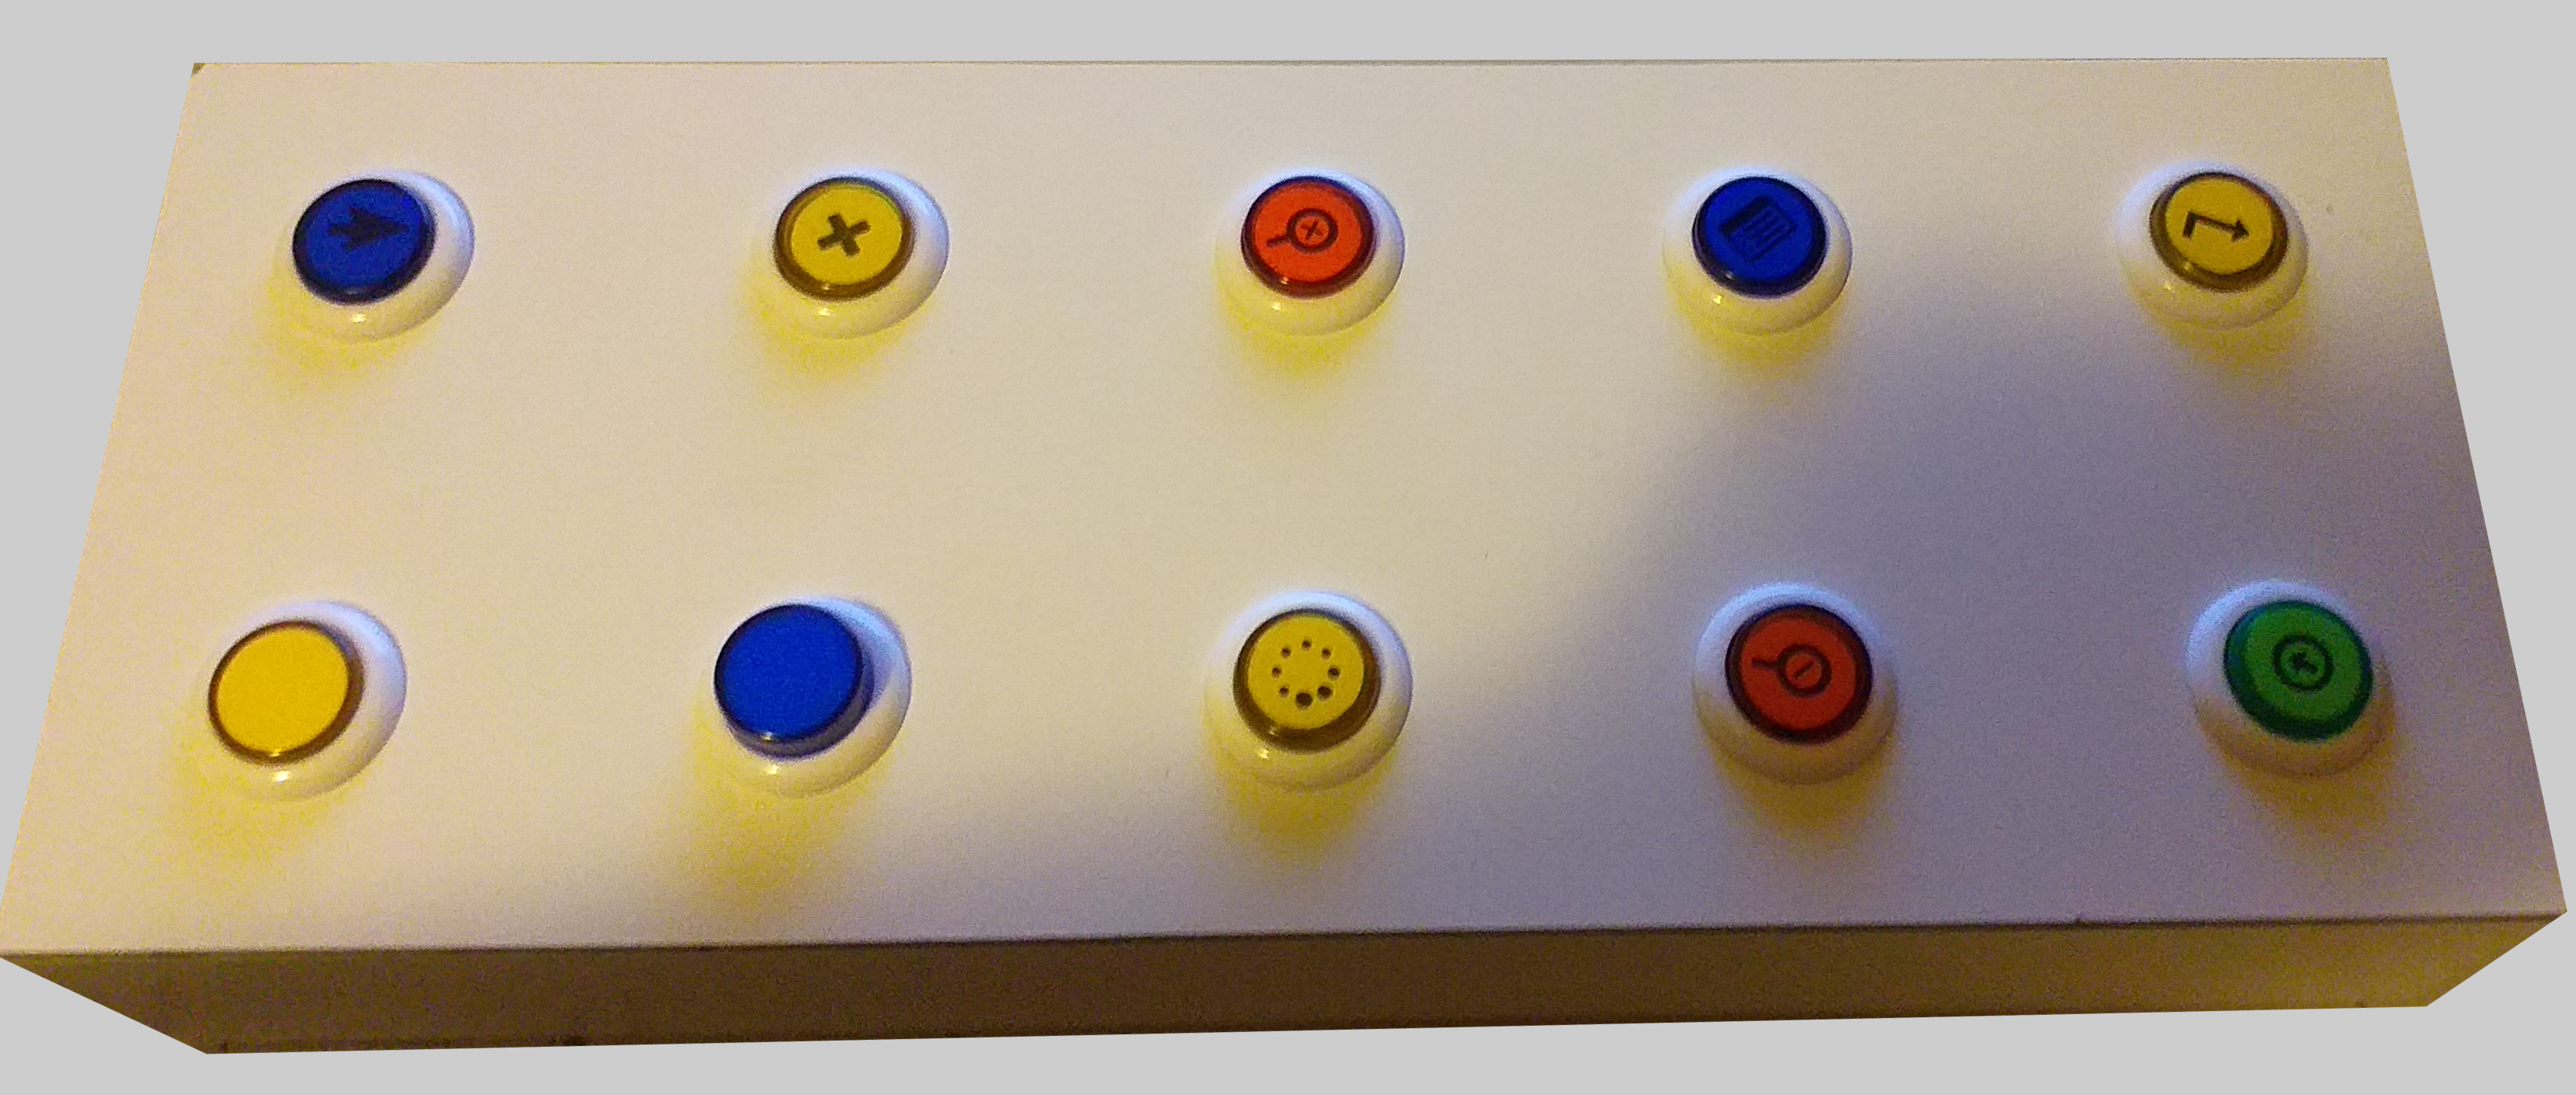
\includegraphics[width=0.8\textwidth]{./img/img-1.png}
		\caption{Controle com botões de comandos montado}
		\label{img:img-1}
\end{figure}

\begin{figure}[H]
	\centering
		\includegraphics[width=0.8\textwidth]{./img/img-10.jpg}
		\caption{Controle com manche montado}
		\label{img:img-10}
\end{figure}

A ligação dos botões foi desenhada no site da tinkercad (Figura \ref{img:img-19}), o mesmo pode ser baixado no MAVERICK,.... . O resistor que foi utilizado é um simples de 650 Khoms, serão necessários 4 deles e alguns fios.

\begin{figure}[H]
	\centering
		\includegraphics[width=0.8\textwidth]{./img/img-19.png}
		\caption{Desenho da ligação dos botões dos controles}
		\label{img:img-19}
\end{figure}

Após feita a montagem da estrutura e ligação dos botões ao ARDUINO®, basta conecta-lo no computador, e o drive será instalado automaticamente. Após a instalação, utilizando o Antimicro ou Xpadder, deve ser configurado as funções de cada botão dos controles.

Funções como aumentar ou diminuir o \emph{zoom}, click direito e esquerdo do \emph{mouse}, fechar a janela atual do sistema operacional, abrir o teclado virtual, movimentação do ponteiro do \emph{mouse}, entre outras funções são possíveis de serem configuradas.
As funções podem ser configuradas de acordo com o perfil do usuario, por exemplo, um usuario que acessa mais a internet, certamente usaria mais as funções de:

\begin{itemize}
\item CTRL + T (Abrir uma nova guia)
\item CTRL + W (Fechar a guia atual)
\item F5 (Recarregar a pagina)
\item \emph{UP} (Subir o \emph{scroll} da tela)
\item \emph{DOWN} (Descer a \emph{scroll} da tela)
\item Abrir teclado virtual
\item \emph{Zoom} +
\item \emph{Zoom} -
\item Clique direito do \emph{mouse}
\item Clique esquerdo do \emph{mouse}
\item Movimentação do mouse
\end{itemize}

Já um usuario que utiliza um software especifico pode configurar para que os controles usem os atalhos do software.

\chapter{Conclusão}

O desenvolvimento do presente estudo possibilitou uma análise de como é a construção de um controle voltado para tecnologias assistivas. Além disso, também permitiu conhecer um pouco mais sobre as areas que envolvem essa construção, e como ela se aplica na sociedade.

Os testes com usuarios não foram realizados, pois para isso é necessário passar pelo comitê de ética, após aprovado podem ser feitos os testes necessários. Como essa aprovação não é simples e acaba sendo demorada, não foi possivel ter a aprovação até a data final de entrega do trabalho.

Para trabalhos futuros pode ser feita a separação dos botões em módulos, para que o usuario ajuste como preferir em sua mesa. Também pode ser reduzido a altura dos controles, utilizando botões com alturas menores.

% ---
% Finaliza a parte no bookmark do PDF, para que se inicie o bookmark na raiz
% ---
\bookmarksetup{startatroot}%
% ---






% ----------------------------------------------------------
% ELEMENTOS PÓS-TEXTUAIS
% ----------------------------------------------------------
\postextual


% ----------------------------------------------------------
% Referências bibliográficas
% ----------------------------------------------------------
%\bibliography{abntex2-modelo-references}

\bibliography{bibliografias}



% ----------------------------------------------------------
% Glossário
% ----------------------------------------------------------
%
% Consulte o manual da classe abntex2 para orientações sobre o glossário.
%
%\glossary

%% ----------------------------------------------------------
%% Apêndices
%% ----------------------------------------------------------
%
%% ---
%% Inicia os apêndices
%% ---
%\begin{apendicesenv}
%
%% Imprime uma página indicando o início dos apêndices
%\partapendices
%
%% ----------------------------------------------------------
%\chapter{Quisque libero justo}
%% ----------------------------------------------------------
%
%\lipsum[50]
%
%% ----------------------------------------------------------
%\chapter{Nullam elementum urna vel imperdiet sodales elit ipsum pharetra ligula
%ac pretium ante justo a nulla curabitur tristique arcu eu metus}
%% ----------------------------------------------------------
%\lipsum[55-57]
%
%\end{apendicesenv}
%% ---
%
%
%% ----------------------------------------------------------
%% Anexos
%% ----------------------------------------------------------


\begin{anexosenv}

% Imprime uma página indicando o início dos anexos
\partanexos

\chapter{Como preparar o ARDUINO® UNO com a biblioteca UnoJoy}

A preparação do ARDUINO® para ser utilizado como um \emph{joystick} com a biblioteca UnoJoy exige que seja feita numa placa que possua o controlador USB ATmega16u2, ou seja outro controlador, como o CH340 não funcionará. A preparação pode ser divida em passos:

Primeiramente vamos baixar os arquivos necessários para fazer a transformação na placa Arduino Uno para Joystick:
%
%Software Flip Atmel:
%
%https://www.microchip.com/DevelopmentTools/ProductDetails/PartNO/FLIP

Software ARDUINO® IDE:

https://www.arduino.cc/en/Main/Software

UnoJoy, BigJoy e Flip:

https://mega.nz/\#!xIhUxC6J!09gFgfu2v187Nu05q7ybW0L6-yoPQdfkY8Axtxx77Xg


1º Passo: Conectar a placa Arduino Uno no Pc e verificar se os drivers estão instalados e se a porta reconheceu a placa Arduino. 

2º Passo: Faça a instalação do flip, dando um duplo clique no instalador do programa e seguindo o que se pede, após ter instalado não será necessário abrir o programa já que a função desse programa é apenas fazer uma comunicação entre o Arduino Uno e o Pc.

3º Passo: Abra a pasta Arduino-big-joystick e faça a extração da pasta compactada Arduino-big-joystick.

4º Passo: Após ter extraído os arquivos, renomeie o arquivo Arduino-big-joystick.hex para UnoJoy.hex, o U e J deixem maiúsculo.

5º Passo: copie o arquivo UnoJoy.hex volte e abra a pasta UnoJoy, abra a pasta UnoJoy outra vez, abra a pasta UnoJoy-master, localize e abra a pasta UnoJoy mais uma vez, agora abra a pasta ATmega8u2Code, agora abra a pasta HexFiles cole e substitua o arquivo UnoJoy.hex.

6º Passo: Volte até a pasta Arduino-big-joystick, abra a mesma e abra a pasta sketchaug19c, dentro desta pasta está a sketch  para fazer a programação no Aduino Uno, abra a sketch e execute dando dois cliques.

7º Passo: Com a sketch aberta vá em ferramentas e verifique se a porta selecionada é a porta que o Arduino Uno está conectado.



\end{anexosenv}


%---------------------------------------------------------------------
% INDICE REMISSIVO
%---------------------------------------------------------------------
\printindex

\end{document}








